% -----------------------------------------------
% Template for SMC 2020
% adapted from previous SMC paper templates
% -----------------------------------------------

\documentclass[dvipsnames, pdftex]{article}
\usepackage{tikz}
% \tikzset{>=latex}
% \tikzstyle{block} = [draw,minimum size=0.5cm]
% \usetikzlibrary{math,arrows,positioning,shapes.geometric, decorations.markings}

\usepackage{smc2020}
\usepackage{times}
\usepackage{ifpdf}
\usepackage[english]{babel}
\usepackage{cite}
\usepackage{multirow}
\usepackage[]{algorithm2e, setspace}
\usepackage{textcomp}
%%%%%%%%%%%%%%%%%%%%%%%% Some useful packages %%%%%%%%%%%%%%%%%%%%%%%%%%%%%%%
%%%%%%%%%%%%%%%%%%%%%%%% See related documentation %%%%%%%%%%%%%%%%%%%%%%%%%%
\usepackage{amsmath} % popular packages from Am. Math. Soc. Please use the 
\usepackage{amssymb}
\usepackage{cases}
% related math environments (split, subequation, cases,
%\usepackage{amsfonts}% multline, etc.)
%\usepackage{bm}      % Bold Math package, defines the command \bf{}
%\usepackage{paralist}% extended list environments
%%subfig.sty is the modern replacement for subfigure.sty. However, subfig.sty 
%%requires and automatically loads caption.sty which overrides class handling 
%%of captions. To prevent this problem, preload caption.sty with caption=false 
%\usepackage[caption=false]{caption}
%\usepackage[font=footnotesize]{subfig}


%user defined variables
\def\papertitle{Real-time Implementation of a Physical Model of the Tromba Marina} %using Finite-Difference Schemes}
\def\firstauthor{Silvin Willemsen}
\def\secondauthor{Stefan Bilbao}
\def\thirdauthor{Michele Ducceschi}
\def\fourthauthor{Stefania Serafin}
% \def\firstauthor{Silvin Willemsen, Stefania Serafin}
% \def\secondauthor{Stefan Bilbao and Michele Ducceschi}

% adds the automatic
% Saves a lot of output space in PDF... after conversion with the distiller
% Delete if you cannot get PS fonts working on your system.

% pdf-tex settings: detect automatically if run by latex or pdflatex
\newif\ifpdf
\ifx\pdfoutput\relax
\else
   \ifcase\pdfoutput
      \pdffalse
   \else
      \pdftrue
\fi

\ifpdf % compiling with pdflatex
  \usepackage[pdftex,
    pdftitle={\papertitle},
    pdfauthor={\firstauthor, \secondauthor, \thirdauthor, \fourthauthor},
    bookmarksnumbered, % use section numbers with bookmarks
    pdfstartview=XYZ % start with zoom=100% instead of full screen; 
                     % especially useful if working with a big screen :-)
   ]{hyperref}
  %\pdfcompresslevel=9

  \usepackage{graphicx}
  % declare the path(s) where your graphic files are and their extensions so 
  %you won't have to specify these with every instance of \includegraphics
  \graphicspath{{./SMC 2020 paper template LaTeX/}}
  \DeclareGraphicsExtensions{.pdf,.jpeg,.png, .eps}

  \usepackage[figure,table]{hypcap}

\else % compiling with latex
  \usepackage[dvips,
    bookmarksnumbered, % use section numbers with bookmarks
    pdfstartview=XYZ % start with zoom=100% instead of full screen
  ]{hyperref}  % hyperrefs are active in the pdf file after conversion

  \usepackage[dvips]{epsfig,graphicx}
  % declare the path(s) where your graphic files are and their extensions so 
  %you won't have to specify these with every instance of \includegraphics
  \graphicspath{{./SMC 2020 paper template LaTeX/}}
  \DeclareGraphicsExtensions{.eps}

  \usepackage[figure,table]{hypcap}
\fi

%setup the hyperref package - make the links black without a surrounding frame
\hypersetup{
    colorlinks,%
    citecolor=black,%
    filecolor=black,%
    linkcolor=black,%
    urlcolor=black
}


% Title.
% ------
\title{\papertitle}

% Authors
% Please note that submissions are NOT anonymous, therefore 
% authors' names have to be VISIBLE in your manuscript. 
%
% Single address
% To use with only one author or several with the same address
% ---------------
%\oneauthor
%   {\firstauthor} {Affiliation1 \\ %
%     {\tt \href{mailto:author1@smcnetwork.org}{author1@smcnetwork.org}}}

%Two addresses
%--------------
\twoauthors
  {\firstauthor{ and }\fourthauthor} {Multisensory Experience Lab, CREATE \\ Aalborg University Copenhagen \\
    {\tt \href{mailto:sil@create.aau.dk}{\{sil, sts\}@create.aau.dk}}}
  {\secondauthor{ and }\thirdauthor} {Acoustics and Audio Group \\ University of Edinburgh \\ %
    {\tt {\{s.bilbao, michele.ducceschi\}@ed.ac.uk}}}

% Three addresses
% --------------
%  \threeauthors
%   {\firstauthor} {Affiliation1 \\ %
%      {\tt \href{mailto:author1@smcnetwork.org}{author1@smcnetwork.org}}}
%   {\secondauthor} {Affiliation2 \\ %
%      {\tt \href{mailto:author2@smcnetwork.org}{author2@smcnetwork.org}}}
%   {\thirdauthor} { Affiliation3 \\ %
%      {\tt \href{mailto:author3@smcnetwork.org}{author3@smcnetwork.org}}}
% \fourauthors
%   {\firstauthor} {Multisensory Experience Lab, CREATE \\ Aalborg University Copenhagen \\ %
%      {\tt \href{mailto:sil@create.aau.dk}{sil@create.aau.dk}}}
%   {\secondauthor} {Acoustics and Audio Group \\ University of Edinburgh \\ %
%      {\tt \href{mailto:s.bilbao@ed.ac.uk}{s.bilbao@ed.ac.uk}}}
%     {\thirdauthor} {Acoustics and Audio Group \\ University of Edinburgh \\ %
%      {\tt \href{mailto:michele.ducceschi@ed.ac.uk}{michele.ducceschi@ed.ac.uk}}}
%   {\fourthauthor} {Multisensory Experience Lab, CREATE \\ Aalborg University Copenhagen \\ %
%      {\tt \href{mailto:sts@create.aau.dk}{sts@create.aau.dk}}}

% ***************************************** the document starts here ***************
\usepackage{xcolor}
\def\SBcomment[#1]{\textcolor{Red}{#1}}
\def\SWcomment[#1]{\textcolor{Bittersweet}{#1}}
\def\MDcomment[#1]{\textcolor{Blue}{#1}}
\def\SScomment[#1]{\textcolor{OliveGreen}{#1}}
\def\stringx{\chi}
\def\ugen{q}
\def\us{u}
\def\um{w}
\def\up{z}

\begin{document}
%
\capstartfalse
\maketitle
\capstarttrue
%
\begin{abstract}
The tromba marina is a medieval bowed monochord instrument. The string of the instrument rests on a rattling bridge that, due to the collision with the body, creates a trumpet-like sound. This paper presents a real-time implementation of a physical model of the tromba marina. The goal of the simulation is to make the instrument accessible to a larger audience. The physical model is implemented using finite-difference time-domain (FDTD) methods and non-iterative collision methods. A real-time implementation of the instrument is also presented. The simulation exhibits brass-like qualities and sounds similar to a real tromba marina, but requires further testing to validate the realism.
%You can place comments in colour if you want :) Like \SBcomment[this (Stefan)], \MDcomment[this (Michele)] or \SScomment[this (Stefania)].
\end{abstract}
%

\section{Introduction}\label{sec:introduction}
The tromba marina (see Figure 
 \ref{fig:tromba}) is a medieval bowed monochord instrument with a long quasi-trapezoidal body and a uniquely fashioned bridge (often called a shoe, because of its shape – see Figure \ref{fig:bridge}). 
 The name of the instrument derives from the fact that {\em tromba} means {\em trumpet} in Italian. A peculiarity of the instrument is that 
 a foot of the bridge is free to rattle against the soundboard in sympathy with the vibrating string. 
 This unusual bridge creates a trumpet-like sound.
 The frequency produced by the instrument is varied by placing the side of the knuckle of the non-dominant hand, lightly, at specific nodal points on the string, in order to select various harmonics of the open string. The dominant hand controls the bow, which is drawn across the string above the non-dominant hand \cite{munrow1976instruments}.
 
  
   \begin{figure}
  \centering
  \includegraphics[width=0.9\columnwidth]{IMG_7980.pdf}
  \caption{The tromba marina from the Danish Music Museum in Copenhagen. }
  \label{fig:tromba}
\end{figure}

  \begin{figure}
  \centering
  \includegraphics[width=0.9\columnwidth]{IMG_7982.JPG}
  \caption{The bridge of the tromba marina from the Danish Music Museum in Copenhagen. The right side is pressed against the body by the string while the left side is free and can rattle against the body.}
  \label{fig:bridge}
\end{figure}

%The tromba marina is therefore a rather unusual instrument with interesting acoustics which is worth investigating using  physical models. 
In this paper, we present a real-time implementation of a physical model of the tromba marina. One of the ultimate goals is the emulation of an instrument that, due to its rarity, is not accessible to a large audience.

Physical modelling for sound synthesis has a long history. Various techniques have been developed to simulate real-world instruments, including mass-spring systems~\cite{cadoz79}, digital waveguides~\cite{smith1992physical} and modal synthesis~\cite{morrison1993mosaic}.
Finite-difference time-domain (FDTD) methods were first used for sound synthesis by Hiller and Ruiz in ~\cite{Ruiz1969, Hiller1971, Hiller2}, later by Chaigne et al. in ~\cite{Chaigne92, Chaigne} and elaborated upon by Bilbao and colleagues in ~\cite{bilbao2009numerical, Bilbao2018:Tutorial}. Compared with other techniques, FDTD methods are more computationally expensive, but easily generalisable and flexible---no assumptions of linearity of travelling wave solutions are employed. Our goal is to implement these techniques in real time and thereby make the simulations playable for the users. For this purpose, we use the expressive Sensel Morph controller \cite{sensel2020}. Other work in real-time control of FDTD methods using this controller includes \cite{Willemsen2019a:SMC2020}. 

The emulation of nonlinear collision interactions in musical instruments normally requires the use of iterative solvers (such as the Newton-Raphson algorithm) \cite{Bilbao15}. For the nonlinear collisions present in the instrument, a method recently proposed in the field of audio by Lopes and Falaize in \cite{Lopes:SMC2020, Falaize2016a:SMC2020, Falaize2016b:SMC2020} and later by Ducceschi and Bilbao in~\cite{Ducceschi2019} allows such iterative methods to be sidestepped. It is thus suited  to creating a real-time implementation of the tromba marina.

This paper is structured as follows: Section \ref{sec:models} presents the models used and Section \ref{sec:disc} shows the discretisation of these. Section \ref{sec:implementation} provides information about implementation, parameter choices, the graphical user interface and control and mapping. Section \ref{sec:resDisc} shows the results and discusses these. Concluding remarks and future work are presented in Section \ref{sec:conclusion}.

\section{Models}\label{sec:models}
The tromba marina can be subdivided into three main components: the string, the bridge and the body. In this section, the partial differential equations (PDEs) of the different components in isolation, under zero-input conditions, will be of the form
\begin{equation}\label{eq:PDEform}
    \mathcal{L}\ugen = 0.
\end{equation}
Here, $\ugen = \ugen(\boldsymbol{x},t)$ represents the state of the component at time $t$ and spatial coordinate $\boldsymbol{x}\in\mathcal{D}$, where the dimensions of domain $\mathcal{D}$ depend on the component at hand. Furthermore, $\mathcal{L}$ is a partial differential operator. (Subscripts `$\text{s}$', `$\text{m}$' and `$\text{p}$' used subsequently indicate that \eqref{eq:PDEform} applies to the string, bridge (mass) or body (plate), respectively.)

\subsection{Bowed Stiff String}
Consider a damped stiff string of length $L$ (m), with domain $\mathcal{D} = \mathcal{D}_\text{s} = [0,L]$ and state variable $\ugen = \us(\stringx,t)$.  
With reference to \eqref{eq:PDEform}, we define the operator $\mathcal{L} = \mathcal{L_\text{s}}$ as \cite{bilbao2009numerical}
\begin{equation}
    \mathcal{L}_\text{s} = \rho_\text{s} A \partial_t^2 - T\partial_\stringx^2 + E_\text{s}I\partial_\stringx^4+2\rho_\text{s} A\sigma_{0,\text{s}}\partial_t-2\rho_\text{s} A\sigma_{1,\text{s}}\partial_t\partial_\stringx^2.
\end{equation}
Here, $\partial_{t}$ and $\partial_{\stringx}$ indicate partial differentiation with respect to $t$ and $\stringx$. The various parameters appear as: material density $\rho_\text{s}$ (kg$\cdot$m$^{-3}$), cross-sectional area $A = \pi r^2$ (m$^2$), radius $r$ (m), tension $T = (2f_{0,\text{s}}L)^2\rho_\text{s}A$ (N),\footnote{Even though this definition for $T$ from the fundamental frequency $f_{0,\text{s}}$ is only valid for a simply supported string without stiffness, the effect of the stiffness eventually chosen for $f_{0,\text{s}}$ is negligible.} %\MDcomment[is this formula valid when you have stiffness? It seems to me that it is only valid under fixed boundary conditions for the wave equation without stiffness]
fundamental frequency $f_{0,\text{s}}$ (s$^{-1}$), Young's modulus $E_\text{s}$ (Pa), area moment of inertia $I=\pi r^4 / 4$ (m$^4$), and loss coefficients $\sigma_{0,\text{s}}$ (s$^{-1}$) and $\sigma_{1,\text{s}}$ (m$^2$/s). We set the boundary conditions to be simply supported so that
\begin{equation}\label{eq:boundary}
    \us = \partial_\stringx^2\us = 0 \quad \text{for} \quad \stringx = 0, L.
\end{equation}
%\SWcomment[In the DAFx paper from last year we wrote $x = 0, L$ instead of $x = {[}0, L{]}$, as -- in this case -- we don't want to specify a domain but single locations instead. Which is correct?]
As the string is excited using a bow, Equation \eqref{eq:PDEform} may be augmented as \cite{bilbao2009numerical}
\begin{equation}\label{eq:bowedString}
    \mathcal{L}_\text{s}\us = -\delta(\stringx-\stringx_\text{b})F_\text{b}\Phi(v_\text{rel}),
\end{equation}
with externally supplied downward bow force $F_\text{b} = F_\text{b}(t)$ (N), spatial Dirac delta function $\delta(\stringx-\stringx_\text{b})$ (m) selecting the bow position $\stringx_\text{b} = \stringx_\text{b}(t)\in \mathcal{D}_\text{s}$ (m) and dimensionless friction characteristic
\begin{equation}
    \Phi(v_\text{rel}) = \sqrt{2a}v_\text{rel}e^{-av_\text{rel}^2+1/2},
\end{equation}
with free parameter $a$. The relative velocity between the string at bow location $\stringx_\text{b}$ and the externally supplied bow velocity $v_\text{b} = v_\text{b}(t)$ (m/s) is defined as
\begin{equation}
    v_\text{rel} = \partial_t\us(\stringx_\text{b},t) - v_\text{b}.
\end{equation}

\subsection{Bridge}
The bridge is modelled as a simple mass-spring-damper system. As this system is point-like, or zero-dimensional, 
the state variable $q = w(t)$ and the definition of domain $\mathcal{D}$ is unnecessary. The operator $\mathcal{L}=\mathcal{L}_\text{m}$ is defined as
\begin{equation}
    \mathcal{L}_\text{m}=M\frac{d^2}{dt^2}+M\omega_0^2+MR\frac{d}{dt},
\end{equation}
with mass $M$ (kg), linear angular frequency of oscillation $\omega_0=2\pi f_{0,\text{m}}$,  (s$^{-1}$), fundamental frequency $f_{0,\text{m}}$ (s$^{-1}$) and damping coefficient $R$ (s$^{-1}$).

\subsection{Body}
The body is simplified to a two-dimensional plate with side-lengths $L_x$ and $L_y$, domain $\mathcal{D} = \mathcal{D}_\text{p} = [0,L_x] \times [0,L_y]$ and state variable $q = \up(x,y,t)$. Using the 2D Laplacian
\begin{equation}\label{eq:laplacian}
    \Delta \triangleq \partial_x^2+\partial_y^2,
\end{equation}
the operator $\mathcal{L} = \mathcal{L}_\text{p}$ can be defined as \cite{bilbao2009numerical}
\begin{equation}
    \mathcal{L}_\text{p} = \rho_\text{p}H\partial_t^2 + D\Delta\Delta +2\rho_\text{p}H\sigma_{0,\text{p}}\partial_t-2\rho_\text{p}H\sigma_{1,\text{p}}\partial_t\Delta,
\end{equation}
with material density $\rho_\text{p}$ (kg$\cdot$m$^{-3}$), plate thickness $H$ (m), stiffness coefficient $D = E_\text{p}H^3/12(1-\nu^2)$, Young's modulus $E_\text{p}$ (Pa), dimensionless Poisson's ratio $\nu$, and loss coefficients $\sigma_{0,\text{p}}$ (s$^{-1}$) and $\sigma_{1,\text{p}}$ (m$^2$/s). The boundary conditions of the plate are set to be clamped so that
\begin{equation}
    \up = {\bf n} \cdot \nabla \up = 0.
\end{equation}
where $\nabla \up$ is the gradient of $\up$, and where ${\bf n}$ indicates a normal to the plate area at the boundary.
\subsection{Collisions}
% \SBcomment[Could really use a diagram here to make sense of the geometry of the rattling bridge ]  \SWcomment[Something like this?]\SBcomment[I guess I meant a diagram of the whole system, showing string/bridge/plate, and all the connection points...] \SWcomment[Something like Figure \ref{fig:trombaSystem}? I thought if would make more sense down there as everything (including the offset) is introduced by then. I thought the first two figures on the first page would clarify how the physical system looked, but maybe it's not clear enough...]
% \SScomment[I thihk it is hard from Figure 3 to see that the b part is rattling. Maybe add the body so it is easier to see that a is attached while b is not?] \SWcomment[Alright, so I guess this makes things more clear :) As I mentioned, there is also a figure more down in the paper (Figure \ref{fig:trombaSystem}) that shows all the important coordinates.]{}
% \SScomment[yes now this is clearer.]
\begin{figure}[ht]
    \centering
    \begin{tikzpicture}
    
    \def\radius{6}; % Radius of the string (>2!)
    \pgfmathsetmacro{\reps}{3}; % How may back-and-forths in the drawing of the springs
    \def\bowSpacing{0.2};
    \def\drawingSpacing{1.5}
    \def\bowWidth{5};
    
    \def\woodWidth{1}; %>0.3
    \def\rattleHeight{0.1};
    \def\bridgeHeight{3};
    \def\bridgeWidth{4};
    \def\cornerRadius{0.15};
    \def\stringWidth{0.2};
    \pgfmathsetmacro{\tinyRadius}{\stringWidth*0.1};
    \pgfmathsetmacro{\stringWidthMinTinyRad}{((\stringWidth-(2*\tinyRadius)))*0.5};
    
    %body
    \draw[-] (-0.5,-\cornerRadius) -- (\bridgeWidth + 2.0 * \woodWidth + 0.6, -\cornerRadius) node[below, midway] (bodyLine) {body};
    
    \def\horShift{0.40};
    \def\width{0.25};
    \foreach \bodyDiag in {-0.5, ...,(\bridgeWidth + 2.0 * \woodWidth + 0.5) * 2.6}
        {
        \pgfmathtruncatemacro{\bD}{\bodyDiag}
        \ifnum \bD<7
            \draw[-] (\bodyDiag * \horShift, -\cornerRadius) -- (\horShift * \bodyDiag - \width, -\cornerRadius -\width);% node (bla) {\bD}; 
            \else
            \ifnum \bD>8
            \draw[-] (\bodyDiag * \horShift, -\cornerRadius) -- (\horShift * \bodyDiag - \width, -\cornerRadius -\width);% node (bla) {\bD}; 
            \fi
            \fi
        }
    
    %straight side
    \draw[-] (0, \bridgeHeight - \cornerRadius) -- (0, 0) node (line) {};
    \draw (0,0) arc(180:270:\cornerRadius cm and \cornerRadius cm);
    \draw (0,\bridgeHeight - \cornerRadius) arc(180:90:\cornerRadius cm and \cornerRadius cm);
    \draw[-] (\cornerRadius, -\cornerRadius) -- (\woodWidth - \cornerRadius, -\cornerRadius) node (line2) {};
    \draw (\woodWidth - \cornerRadius, -\cornerRadius) arc(270:360:\cornerRadius cm and \cornerRadius cm);
    \draw[-] (\woodWidth, 0) -- (\woodWidth, \bridgeHeight - \woodWidth - \cornerRadius) node (line) {};
    \draw (\woodWidth, \bridgeHeight - \woodWidth - \cornerRadius) arc(180:90:\cornerRadius cm and \cornerRadius cm);
    
    %%% string cavity %%%
    
    % define left and right position of the string cavity
    \pgfmathsetmacro{\leftStringPos}{\woodWidth * 0.5 - \stringWidth * 0.5};
    \pgfmathsetmacro{\rightStringPos}{(\woodWidth + \stringWidth) * 0.5};
    
    %line to cavity
    \draw[-] (\cornerRadius, \bridgeHeight) -- (\leftStringPos, \bridgeHeight) node (line) {};
   
    %tiny arc
    \draw (\leftStringPos, \bridgeHeight) arc(90:0:\tinyRadius cm and \tinyRadius cm);
    
    %stringarc
    \draw (\leftStringPos + \tinyRadius, \bridgeHeight - \tinyRadius) arc(180:360:\stringWidthMinTinyRad cm and \stringWidthMinTinyRad cm);
    %tinyarc
    \draw (\rightStringPos - \tinyRadius, \bridgeHeight - \tinyRadius) arc(180:90:\tinyRadius cm and \tinyRadius cm);
    
    % line to rest of bridge
    \draw[-] (\rightStringPos, \bridgeHeight) -- (\woodWidth + \cornerRadius, \bridgeHeight) node (line2) {};
    
    %bottom of arc
    
    \pgfmathsetmacro{\rattle}{\bridgeHeight-\woodWidth-\rattleHeight};
    \draw (\woodWidth + \cornerRadius, \bridgeHeight - \woodWidth) arc(90:0:\bridgeWidth cm and \rattle cm);
    %% bottom of rattle
    
    %cur x-pos
    \pgfmathparse{\woodWidth + \bridgeWidth + \cornerRadius};
    \draw (\pgfmathresult, \rattleHeight) arc(180:270:\cornerRadius cm and \cornerRadius cm);
    \draw[-] (\pgfmathresult + \cornerRadius, -\cornerRadius+\rattleHeight) -- ({\woodWidth + \bridgeWidth + \woodWidth}, -\cornerRadius+\rattleHeight) node (line) {};
    \pgfmathparse{2.0 * \woodWidth + \bridgeWidth};
    \draw (\pgfmathresult, -\cornerRadius+\rattleHeight) arc(270:360:\cornerRadius cm and \cornerRadius cm);
    
    %% top part of the arc
    \pgfmathsetmacro{\toparc}{\bridgeWidth + \woodWidth};
    \pgfmathsetmacro{\yTopArc}{\bridgeHeight - \rattleHeight};
    \pgfmathparse{\bridgeWidth + 2.0*\woodWidth + \cornerRadius};
    \draw (\pgfmathresult, \rattleHeight) arc(0:90:\toparc cm and \yTopArc cm);
    
    
    %%%% Annotations %%%%
    \def\arrowLength{0.5};
    \draw[<-] (\woodWidth + 0.1, 0.05) -- (\woodWidth + 0.1 + \arrowLength, 0.05) node [right] (TextNode) {a)};
    \draw[<-] (\woodWidth + \cornerRadius + \bridgeWidth - 0.1 , \rattleHeight) -- (\woodWidth + \cornerRadius + \bridgeWidth - 0.1 - \arrowLength, \rattleHeight) node [left] (TextNode) {b)};
    \draw[<-] (\woodWidth * 0.5, \bridgeHeight + 0.05) |- (\woodWidth, \bridgeHeight + 0.25) node [right] (TextNode) {c)};
    \end{tikzpicture}
    \caption{Diagram of the bridge while rattling (view from top of the tromba marina). Indicated are: a) the pivoting point always in contact with the body, b) the rattling point colliding with the body (currently not colliding), and c) the string cavity straight above the middle of the pivoting point.}
    \label{fig:bridgeDiagram}
\end{figure}
%
It can be argued that the greatest contributor to the characteristic sound of the tromba marina is the rattling bridge colliding with the body. A diagram of the bridge with important parts highlighted can be found in Figure \ref{fig:bridgeDiagram}. A collision can be modelled by including a term to the PDEs mentioned above describing the potential energy of the system (further referred to as \textit{the potential}) \cite{Ducceschi2019}. For the bridge-body (mass-plate) interaction this potential is defined as follows %\MDcomment[watch out: $\phi$ is a function of $\eta$ only ... not time. ]{}\SWcomment[when discretising it, I ran into the fact that $\eta$ is time-dependent, but of course, its value doesn't changed based on time, only based on $\eta$]{}
\begin{equation}\label{eq:potential}
    \phi_\text{mp}(\eta_\text{mp}) = \frac{K_\text{mp}}{\alpha_\text{mp}+1}[\eta_\text{mp}]_+^{\alpha_\text{mp}+1},
\end{equation}
\begin{equation*}
    K_\text{mp}>0, \quad \alpha_\text{mp}\geq 1, \quad \eta_\text{mp}\triangleq \up(x_\text{mp},y_\text{mp},t) - \um(t)
\end{equation*}
where $K_\text{mp}$ is the collision stiffness (N/m if $\alpha_\text{mp} = 1$), $\alpha_\text{mp}$ is the dimensionless nonlinear collision coefficient, and $\eta_\text{mp} = \eta_\text{mp}(t)$ is the distance between the rattling part of the bridge and the body at the point of collision (m). Furthermore, $[\eta_\text{mp}]_+ = 0.5(\eta_\text{mp}+|\eta_\text{mp}|)$ is the positive part of $\eta_\text{mp}$. Note that penalty methods are employed here, where a positive $\eta_\text{mp}$, i.e., interpenetration of the colliding objects, is intended \cite{bilbao2014:SMC2020}. The term which can then be included in the PDEs is $\phi_\text{mp}' = d\phi_\text{mp}/d\eta_\text{mp}$. As described in \cite{Falaize2016a:SMC2020, Falaize2016b:SMC2020, Lopes:SMC2020, Ducceschi2019}, using this form of the potential requires using iterative methods for solving its discrete counterpart. In \cite{Ducceschi2019}, the authors propose to rewrite the potential to
\begin{equation}
    \psi = \sqrt{2\phi},
\end{equation}
and the term included in the PDEs to
\begin{equation}\label{eq:phiToPsi}
    \phi' = \psi\psi' = \psi\frac{d\psi}{d\eta}\  \xrightarrow{\text{chain rule}}\ \psi\frac{\dot \psi}{\dot \eta}\ ,
\end{equation}
where the dot above $\psi$ and $\phi$ denotes a single time derivative. Equation \eqref{eq:phiToPsi}, as can be seen in Section \ref{sec:disc}, leads to guaranteed stable and explicitly computable simulation algorithms without the need for iterative solvers. 

As the string rests on the bridge, the interaction between these components needs to be modelled as well. Even though the bridge-body interaction is perpendicular to the string-bridge interaction, we can model them as being parallel, assuming that a ``horizontal" movement of the string causes a ``vertical" movement of the rattling part of the bridge. We can use an alternative version of the potential in Equation~\eqref{eq:potential} described in \cite{Bilbao2019} to make the collision two-sided acting as a connection:
\begin{equation}\label{eq:phiConnection}
    \phi_\text{sm}(\eta_\text{sm}) = \frac{K_\text{sm}}{\alpha_\text{sm}+1}|\eta_\text{sm}|^{\alpha_\text{sm}+1},
\end{equation}
%
\begin{equation*}
    K_\text{sm}>0, \quad \alpha_\text{sm}\geq 1, \quad \eta_\text{sm}\triangleq \um(t) - \us(\stringx_\text{sm},t)
\end{equation*}
where $\eta_\text{sm} = \eta_\text{sm}(t)$ is the distance between the string at the location of the bridge and the bridge itself. 

\subsection{Complete System}

A complete system for the tromba marina may be written, in continuous-time as:
\begin{subnumcases}{\label{eq:fullSystem}}
% \begin{aligned}
    \mathcal{L}_\text{s}\us &$=-\delta(\stringx-\stringx_\text{b})F_\text{b}\Phi(v_\text{rel})$ \label{eq:stringPotential}\\
    & $\quad\ \,\!\!+\  \delta(\stringx-\stringx_\text{sm})\psi_\text{sm}\psi_\text{sm}'$\nonumber\\
    \mathcal{L}_\text{m}\um &$= -\psi_\text{sm}\psi_\text{sm}' + \psi_\text{mp}\psi_\text{mp}',$\label{eq:massPotential}\\
    \mathcal{L}_\text{p}\up &$= -\delta(x-x_\text{mp}, y-y_\text{mp})\psi_\text{mp}\psi_\text{mp}',$\qquad\label{eq:platePotential}\\
    \eta_\text{sm} &$= \um(t) - \us(\stringx_\text{sm}, t),$\\
    \eta_\text{mp} &$=  \up(x_\text{mp}, y_\text{mp}, t) - \um(t),$
% \end{aligned}
\end{subnumcases}
%\MDcomment[There is a little confusion that may arise in the notation, as $x$ is used to indicate the coordinate on the string, and on the plate ... but those are two different x's. You could use a different letter for the string, perhaps a greek letter? say $\chi$]{}
where $\stringx_\text{sm} \in \mathcal{D}_\text{s}$ is the location of the bridge along the string and $(x_\text{mp}, y_\text{mp}) \in \mathcal{D}_\text{p}$ is the location on the body with which the bridge collides. 
%Note that the same symbol $x$ for is used for both the string and the body, but are completely independent as they apply to the domains of their respective model. 
%Furthermore, to avoid confusion between the coordinate along the string and the x-coordinate on the plate, we use $u(\chi,t)$ for the string.
%Note that the potentials belonging to a single collision in the above system have inverse signs as the collision force acts inversely on the two components. \textbf{not sure if this sentence is necessary, and otherwise rewrite..}\MDcomment[I think that this sentence is unncessary ... the signs are correct because the force is always acting against the displacement (or you can do energy analysis, and you'll get the same answer)]{}

% \SBcomment[OK, here I would use a different coordinate $\eta$ or something for the spatial coordinate along the string, which is not the same as $x$ for the plate...this needs to be changed in the earlier sections as well. ] \SWcomment[Could I use something that looks more like an `x' (such as $\text{\it x}$)?]{} \SBcomment[It would be good to pick something without a subscript if possible. Maybe $\xi$ for the string?] \SWcomment[I'm not sure what you mean with ``without a subscript".. Do you mean regular character? $\text{\it x}$ is without a subscript at this point and a different symbol than $x$. If you think they look too much alike, I could use $\xi$, but I feel that using anything different than an $x$-like symbol for space would be counterintuitive (for me and also perhaps the reader)]\SBcomment[OK, but the difference between $x$ and $\text{\it x}$ is going to be even more confusing I think...] \SWcomment[Michele proposed $\chi$ earlier. Maybe I'll do that instead.. or $X$?]{}\SBcomment[$\chi$ is a good choice...]

\section{Discretisation}\label{sec:disc}
System \eqref{eq:fullSystem} is discretised using FDTD methods. These methods subdivide the continuous system in grid points in space and samples %\SWcomment[or should I say indices here?] 
in time. Before going into the discretisation of the models, and collision and connection terms in the system described in \eqref{eq:fullSystem}, some finite difference operators are introduced.

\subsection{Operators}
The identity and temporal shift operators are defined as
\begin{equation}
    1\eta^n = \eta^n, \quad e_{t+}\eta^n = \eta^{n+1}, \quad e_{t-}\eta^n = \eta^{n-1}.
\end{equation}
% similarly for interleaved grid points
% \begin{equation}
%     e_{t+}\psi^{n-1/2} = \psi^{n+1/2}, \quad e_{t-}\psi^{n+1/2} = \psi^{n-1/2}.
% \end{equation}
Using these, the operators for the forward, backward and centered time differences can be defined as
\begin{equation}\label{eq:discTimeOperators}
    \delta_{t+} = \frac{e_{t+} - 1}{k},\ \delta_{t-} = \frac{1 - e_{t-}}{k},\ \delta_{t\cdot} = \frac{e_{t+}-e_{t-}}{2k},
\end{equation}
and are all approximations to a first-order time derivative. Furthermore, forwards and backwards averaging operators are defined as
\begin{equation}
    \mu_{t+} = \frac{e_{t+} + 1}{2}, \quad \mu_{t-} = \frac{1 + e_{t-}}{2}.
\end{equation}
and can be used to describe interleaved grid points $n+1/2$ and $n-1/2$ respectively.

\subsection{Discrete Models}
To approximate the state of a system in isolation we use
\begin{equation}\label{eq:generalDisc}
    \ugen(\boldsymbol{x},t) \approx \ugen^n_{\boldsymbol{l}}, 
\end{equation} 
where grid function $\ugen^n_{\boldsymbol{l}}$ is a discrete approximation to $\ugen({\boldsymbol{x}},t)$ at $t=nk$ with time step $k$ (s), time index $n\geq 0$ and grid location $\boldsymbol{l}$ that depends on domain $\mathcal{D}$ of the system at hand. In the case of the string, we use $\stringx=lh_\text{s}$ with grid spacing $h_\text{s}$ (m), $\boldsymbol{l} = l \in [0,\hdots, N]$ and total number of grid points $N=L/h_\text{s}$ to yield $\us(\stringx,t) \approx \us_l^n$.
% 
% As the bridge is point-like, a definition of $\boldsymbol{l}$ is unnecessary and $\um(t) \approx \um^n$.\SBcomment[Can omit this] 

In the case of the body, we use $x=lh_\text{p}$ and $y=mh_\text{p}$ to get $\up(x, y, t) \approx \up_{(l,m)}^n$ where $\boldsymbol{l} = (l,m)$ with $l\in[0,\hdots,N_x]$ and $m\in[0,\hdots,N_y]$. Here, $N_x = L_x / h_\text{p}$ and $N_y = L_y / h_\text{p}$ are the horizontal and vertical number of grid points respectively with grid spacing $h_\text{p}$ (m).

%  = \boldsymbol{l}h$ with grid spacing $h$ and $\boldsymbol{l}$ describes the coordinates of the points in an isolated system (string, mass or plate) and
 
The discretisation of and expansion of operator $\mathcal{L}\approx \ell$ in the case of stiff strings, mass-spring systems and plates using FDTD methods are well covered in the literature \cite{bilbao2009numerical} and will not be described in detail in this paper. To obtain the highest accuracy possible while keeping the system explicit (except for the bow), centered differences -- which are second-order accurate -- have been chosen where possible. 

For stability, grid spacings $h_\text{s}$ and $h_\text{p}$ should satisfy the conditions below. In the case of the damped stiff string,
\begin{equation}
    h_\text{s} \geq \sqrt{\frac{c^2k^2+4\sigma_{1,\text{s}}k+\sqrt{(c^2k^2+4\sigma_{1,\text{s}}k)^2+16\kappa_\text{s}^2k^2}}{2}},
\end{equation}
with wave speed $c = \sqrt{T/\rho_\text{s}A}$ and stiffness coefficient $\kappa_\text{s} = \sqrt{E_\text{s}I/\rho_\text{s}A}$ and in the case of the plate,
\begin{equation}\label{eq:gridSpacingPlate}
    h_\text{p} \geq 2\sqrt{k\left(\sigma_{1,\text{s}} + \sqrt{\kappa_\text{p}^2 + \sigma_{1,\text{s}}^2}\right)}\ ,
\end{equation}
with stiffness coefficient $\kappa_\text{p} = \sqrt{D/\rho_\text{p}H}$. The closer the grid spacings are to these conditions, the higher the accuracy of the approximation. 

In order to discretise the Dirac delta functions found in system \eqref{eq:fullSystem} we introduce a spreading operator $J(\boldsymbol{x}_\text{c})$ that applies a force to coordinate $\boldsymbol{x}_\text{c}$, which, in the simplest case, is defined as \cite{bilbao2009numerical}
\begin{equation}
   J(\boldsymbol{x}_\text{c}) = \begin{cases}
       \frac{1}{h^d}, & \boldsymbol{l} = \boldsymbol{l}_\text{c} = \text{round}(\boldsymbol{x}_\text{c} / h)\\
       0, & \text{otherwise}
   \end{cases}
\end{equation}
Here, $d$ is the number of dimensions of domain $\mathcal{D}$ that $\boldsymbol{x}$ is defined for, i.e., $d=0$ for the bridge, $d=1$ for the string, and $d=2$ for the plate. For finer control, a cubic spreading operator $J_3$ can be introduced \cite{bilbao2009numerical}. This is used for the bowing term in Equation \eqref{eq:bowedString}, which is discretised as follows
\begin{equation}
    \ell_\text{s}\us^n_l = -J_3(\stringx_\text{b})F_\text{b}^n\phi(v_\text{rel}^n)
\end{equation}
where, using the centered difference operator from Equation \eqref{eq:discTimeOperators},
\begin{equation}\label{eq:discBow}
    v_\text{rel}^n = \delta_{t\cdot}\us_{l_\text{b}}^n-v_\text{b}^n,
\end{equation}
with coordinate $l_\text{b} = \stringx_\text{b}/h_\text{s}$. Equation \eqref{eq:discBow} needs to be calculated using iterative methods.

\subsection{Collisions using Non-Iterative Methods}

For the discrete-time definitions of the potential in \eqref{eq:phiToPsi} we can use 
\begin{equation}\label{eq:discretePsi}
    \psi\approx \mu_{t+}\psi^{n-1/2}\quad \text{and} \quad \psi' \approx \frac{\delta_{t+}\psi^{n-1/2}}{\delta_{t\cdot}\eta^n},
\end{equation}
% \begin{equation}
%     g^n = \frac{\delta_{t+}\psi^{n-1/2}}{\delta_{t\cdot}\eta^n},
% \end{equation}
where $\psi$ at interleaved grid point $n-1/2$ is defined as
\begin{equation}
    \psi^{n-1/2} = \mu_{t-}\psi^n.
\end{equation}
Note that applying a forward or backward difference operator to an interleaved grid -- such as $\delta_{t+}\psi^{n-1/2}$ in Equation \eqref{eq:discretePsi} -- is second-order accurate.

For a system that has a single (upward) collision we get
\begin{equation}\label{eq:dummySystem}
    \ell \ugen^n_{\boldsymbol{l}} = J(\boldsymbol{x}_\text{c})\left(\mu_{t+}\psi^{n-1/2}\right)\frac{\delta_{t+}\psi^{n-1/2}}{\delta_{t\cdot}\eta^n}.
\end{equation}
Here, we use the identity 
\begin{equation}\label{eq:identity}
    \mu_{t+}\psi^{n-1/2} = \frac{k}{2}\delta_{t+}\psi^{n-1/2}-\psi^{n-1/2}
\end{equation}
and define
\begin{equation}\label{eq:gn}
    %\psi' \approx 
    g^n = \frac{\delta_{t+}\psi^{n-1/2}}{\delta_{t\cdot}\eta^n},
\end{equation}
which can be rewritten to
\begin{equation}\label{eq:gnRewritten}
    \delta_{t+}\psi^{n-1/2} = g^n\delta_{t\cdot}\eta^n.
\end{equation}
Then, inserting \eqref{eq:gnRewritten} into \eqref{eq:identity} and this together with \eqref{eq:gn} into \eqref{eq:dummySystem} we get
\begin{equation}\label{eq:inserted}
    \ell \ugen^n_{\boldsymbol{l}} = J(\boldsymbol{x}_\text{c})\left(\frac{k}{2}g^n\delta_{t\cdot}\eta^n-\psi^{n-1/2}\right)g^n
\end{equation}
where $g^n$ may be explicitly calculated using the analytic expressions for $\psi$ and $\phi$ \cite{Ducceschi2019}:
\begin{equation}\label{eq:analytic}
    g^n = \psi'\bigg\rvert_{\eta=\eta^n} = \frac{\phi'}{\sqrt{2\phi}}\bigg\rvert_{\eta=\eta^n}.
\end{equation}
Numerical stability of this scheme is shown in \cite{Ducceschi2019}. When writing out \eqref{eq:analytic} we can obtain definitions for $g_\text{sm}^n$ using \eqref{eq:phiConnection}
\begin{equation}\label{eq:gnSM}
    g_\text{sm}^n =\text{sgn}(\eta_\text{sm}^n)\sqrt{\frac{K_\text{sm}(\alpha_\text{sm}+1)}{2}}|\eta_\text{sm}^n|^{\frac{\alpha_\text{sm}-1}{2}}\ ,
\end{equation}
and $g_\text{mp}^n$ using \eqref{eq:potential}
\begin{equation}\label{eq:gnMP}
    g_\text{mp}^n =\sqrt{\frac{K_\text{mp}(\alpha_\text{mp} + 1)}{2}} [\eta_\text{mp}^n]_+^{\frac{\alpha_\text{mp} - 1}{2}}\ .
\end{equation} 

\subsection{Complete Discrete System}
Introducing for brevity,
\begin{equation}\label{eq:qn}
    \xi^n  = \frac{k}{2}g^n\delta_{t\cdot}\eta^n-\psi^{n-1/2},
\end{equation}
the discrete counterpart of the complete system described in \eqref{eq:fullSystem} will be
\begin{subnumcases}{\label{eq:fullSystemDisc}}
    % \begin{aligned}
        \ell_\text{s}\us_l^n &$=-J_3(\stringx_\text{b}^n)F_\text{b}\Phi(v_\text{rel}^n)+J(\stringx_\text{sm})\xi_\text{sm}^ng_\text{sm}^n,\qquad\ \ \;$\label{eq:stringDisc}\\
        \ell_\text{m}\um^n &$= -\xi_\text{sm}^ng_\text{sm}^n+\xi_\text{mp}^ng_\text{mp}^n,$\label{eq:massDisc}\\
        \ell_\text{p}\up_{(l,m)}^n\hspace{-3.0cm} &$= -J(x_\text{mp}, y_\text{mp})\xi_\text{mp}^ng_\text{mp}^n,$\qquad\label{eq:plateDisc}\\
        \eta_\text{sm}^n &$= \um^n - \us^n_{l_\text{sm}},$\label{eq:etaSMDisc}\\
        \eta_\text{mp}^n &$=  \up_{(l_\text{mp}, m_\text{mp})}^n - \um^n,$\label{eq:etaMPDisc}
    % \end{aligned}
\end{subnumcases}
% \begin{subnumcases}{\label{eq:fullSystemDisc}}
%     % \begin{aligned}
%         \ell_\text{s}u_{l}^n &$=-J(\stringx_\text{b}^n)F_\text{b}\Phi(v_\text{rel}^n)$\label{eq:stringPotential}\\
%         & $\quad\ \,\!\!+\  J(\stringx_\text{sm})\left(\frac{k}{2}\delta_{t\cdot}\eta_\text{sm}^n-\psi_\text{sm}^{n-1/2}\right)g_\text{sm}^n,$\nonumber\\
%         \ell_\text{m}\um^n &$= -\left(\frac{k}{2}\delta_{t\cdot}\eta_\text{sm}^n-\psi_\text{sm}^{n-1/2}\right)g_\text{sm}^n$\\
%         &$\quad\ \,\!\!+\left(\frac{k}{2}\delta_{t\cdot}\eta_\text{mp}^n-\psi_\text{mp}^{n-1/2}\right)g_\text{mp}^n,$\label{eq:massPotential}\\
%         \ell_\text{p}\up_{(l,m)}^n\hspace{-3.0cm} &$= -J(x_\text{mp}, y_\text{mp})$\\
%         &$\quad\ \,\!\!\cdot\left(\frac{k}{2}\delta_{t\cdot}\eta_\text{mp}^n-\psi_\text{mp}^{n-1/2}\right)g_\text{mp}^n,$\qquad\label{eq:platePotential}\\
%         \eta_\text{sm}^n &$= \um^n - \us^n_{l_\text{sm}},$\\
%         \eta_\text{mp}^n &$=  \up_{(x_\text{mp}, y_\text{mp})}^n - \um^n,$
%     % \end{aligned}
% \end{subnumcases}
\\
where discrete counterparts of connection and collision locations in Equations \eqref{eq:etaSMDisc} and \eqref{eq:etaMPDisc} are described as $l_\text{sm} = \stringx_\text{sm}/h_\text{s}$ and $(l_\text{mp}, m_\text{mp}) = (x_\text{mp}/h_\text{p}, y_\text{mp}/h_\text{p})$. This leaves us with two different types of update equations, one where $\ugen^{n+1}_{\boldsymbol{l}}$ is calculated and one where $\psi^{n+1/2}$ is calculated.

One might think that due to the centered differences $\delta_{t\cdot}\eta^n$ still present in Equation \eqref{eq:qn}, our system remains implicit, but as we can insert the definitions for Equations \eqref{eq:etaSMDisc} and \eqref{eq:etaMPDisc} evaluated at the next time index $n+1$, which are already present in $\ell_\text{s}\us_l^n$, $\ell_\text{m}\um^n$ and $\ell_\text{p}\up_{(l,m)}^n$, the Equations in \eqref{eq:fullSystemDisc} reduce to a system of linear equations that can be solved by a single division. %\SWcomment[Does this make sense? I thought to add this paragraph to emphasise that the system is now actually explicit.]

\section{Implementation}\label{sec:implementation}
The real-time implementation of the system has been done in C++ using the JUCE framework \cite{JUCE2020} and will be controlled using the Sensel Morph (or simply Sensel) -- an expressive touch controller. A demo of the application can be found in \cite{youtubeDemo:SMC2020}. This section will first elaborate some important considerations regarding the setup of the system. Then, the algorithm together with the parameter design will be presented.  Finally, the graphical user interface (GUI) will be detailed together with the Sensel and its mapping to the application.

\subsection{Introducing an Offset}
Firstly, for more realistic and expressive sounds, we model the bridge -- and with that, the string -- to rest slightly above the body. Expanding $\ell_\text{m}\um^n$ in \eqref{eq:massDisc} and including the offset yields
\begin{equation}\label{eq:offset}
    \ell_\text{m}\um^n \Rightarrow M\delta_{tt}\um^n+M\omega_0^2(\um^n-\um_\text{off})+MR\delta_{t\cdot}\um^n
\end{equation}
where $\um_\text{off} \geq 0$ is a predefined offset between the body and the bridge. Furthermore, the second-order time derivative can be defined from the definitions in \eqref{eq:discTimeOperators} as
\begin{equation}
    \delta_{tt} = \delta_{t+}\delta_{t-}\ .
\end{equation}
The boundary condition of the string defined in Equation \eqref{eq:boundary} will also change depending on the bridge offset:
\begin{equation}\label{eq:newBoundary}
    \us = \um_\text{off}\quad \text{and} \quad \partial_\stringx^2\us=0.
\end{equation}

\subsection{Pitch Control}
Secondly, as briefly mentioned in Section \ref{sec:introduction}, the way that different pitches are played on the tromba marina, is to slightly rest a knuckle or finger on nodal points along the string to induce harmonics. Thus, a damping finger is implemented. Using the cubic interpolation operator $I_3$ \cite{bilbao2009numerical}, Equation \eqref{eq:stringDisc} can be extended to
\begin{gather}\label{eq:dampingFinger}
    \ell_\text{s} \us_l^n = \hdots - J_3(\stringx_\text{f})I_3(\stringx_\text{f})\sigma_\text{f}(\us^n_l-\um_\text{off}),\\
   \text{where} \quad 0\leq \sigma_\text{f} \leq 1,\nonumber
\end{gather}
which essentially subtracts its own state at location $\stringx_\text{f} \in [0,0.5\stringx_\text{sm}]$ according to the damping coefficient $\sigma_\text{f}$ (kg$ \cdot$ s$^{-2}$) applied. As done in \cite{Willemsen2019a:SMC2020}, the fractional part used in the spreading operator ($\alpha_\text{i} = \stringx_\text{f}/h - \text{floor}(\stringx_\text{f}/h)$) is raised to the 7th power as it has been found to scale finger position to pitch more properly in the context of FDTD. As the string is bowed above the damping finger (at the other side of the rattling bridge) it is essential that the energy from the bow reaches the rattling bridge, which is still the case for lower values of $\sigma_\text{f}$. A more realistic approach that could be investigated is to model the finger as a mass colliding with the string, rather than imposing the damping directly to the state of the string as presented here.

A schematic plot of the full system, including the offset described in Equations \eqref{eq:offset} and \eqref{eq:newBoundary} and the damping finger from Equation \eqref{eq:dampingFinger} can be found in Figure \ref{fig:trombaSystem}.

\begin{figure}[t]
  \centering
  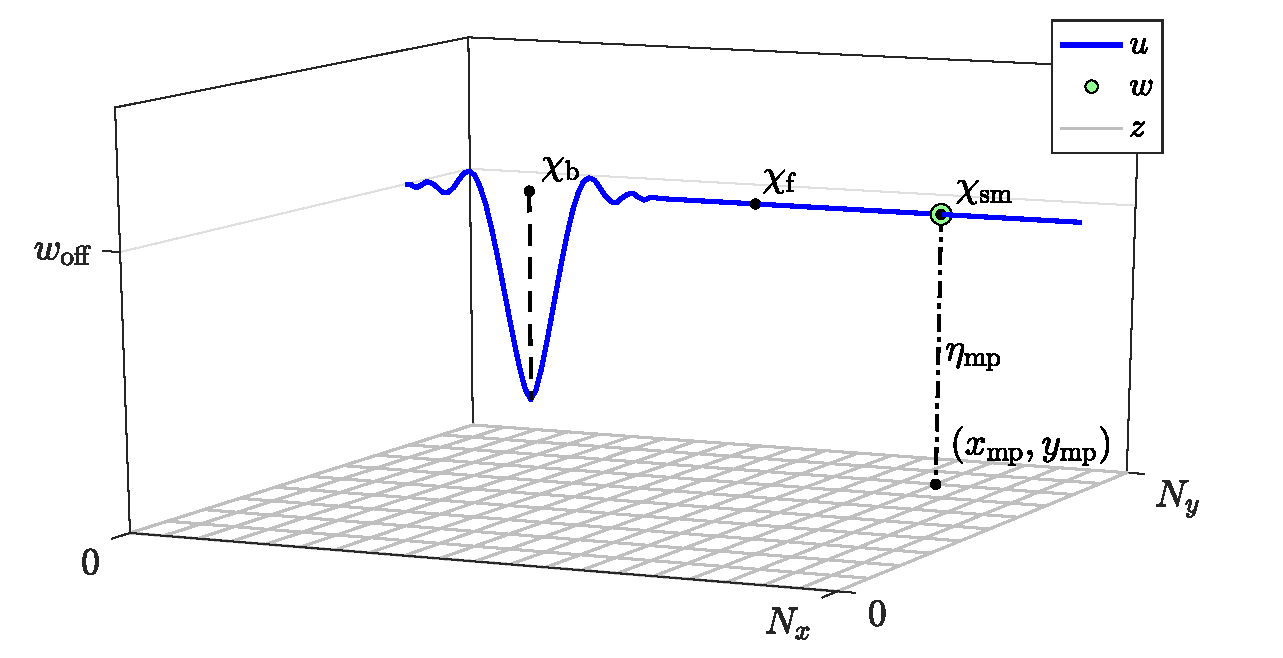
\includegraphics[width=1.0\columnwidth]{trombaSystem.eps}
  \caption{The virtual system in \eqref{eq:fullSystemDisc} including the offset in Equation \eqref{eq:offset} and the damping finger in Equation \eqref{eq:dampingFinger}, with different important coordinates highlighted. Note that $\eta_\text{sm}$ (Equation \eqref{eq:etaSMDisc}) is not shown as it is close to 0 at all times.}
  \label{fig:trombaSystem}
\end{figure}


\subsection{Other Considerations}
Realistic initialisation of both $\eta_\text{sm}$ and $\eta_\text{mp}$ is essential. In this case (at $n=0$) $\eta_\text{sm}^0 = 0$ and $\eta_\text{mp}^0 \leq 0$ so that no collision is present at initialisation.% If this is not done, the value for the potential at the previous time step $\psi^{n-1/2}$ would need to have a value, but doesn't. 

After $h_\text{p}$ is calculated in Equation \eqref{eq:gridSpacingPlate}, we check whether it is smaller than a set value $h_{\text{p},\text{min}} = 0.01$. This reduces the quality of the model, but increases the speed, ultimately allowing for real-time implementation.

\subsection{Order of Calculation} 
The order of calculation is shown in the pseudocode in Algorithm \ref{alg:calcOrder}. In theory, in order to iteratively calculate the bow force, the collision and connection forces should be included in this. %\SWcomment[Hmm.. but the rest of the system is explicit. Shouldn't the system be calculated in its entirety before the NR calculation?] 
However, as the string is practically never bowed at the bridge position $\stringx_\text{sm}$, these can be calculated independently.
%
\begin{algorithm}[ht]
\centering
\fbox{\parbox{0.9\linewidth}{
\setstretch{1.5}
 \While{application is running}{
 \vspace{0.15cm}
 \begin{minipage}[c]{0.48\linewidth}
1. calculate schemes\\
2. apply bow to string\\
3. apply damping finger\\
4. calculate $g^n_\text{sm}$ and $g^n_\text{mp}$\\
\vspace{-0.2cm}5. calculate collision and
\vspace{-0.2cm}connection forces and add to schemes\\
\vspace{-0.2cm}6. Update states \\
\vspace{-0.2cm}\\
\end{minipage}
\hspace{0.05cm}
\begin{minipage}[c]{0.42\linewidth}
($\ell q$ in Eqs. (\ref{eq:stringDisc}-c))\\
(Eq. \eqref{eq:stringDisc})\\
(Eq. \eqref{eq:dampingFinger})\\
(Eqs. \eqref{eq:gnSM} and \eqref{eq:gnMP})\\
\vspace{-0.2cm}(Eqs. (\ref{eq:stringDisc}-c))\\
\vspace{-0.2cm}\\
\\
\vspace{-0.2cm}$\boldsymbol{\ugen}^{n-1} = \boldsymbol{\ugen}^n$\\
\vspace{-0.2cm}$\boldsymbol{\ugen}^{n} = \boldsymbol{\ugen}^{n+1}$\\
$\boldsymbol{\psi}^{n-1/2} = \boldsymbol{\psi}^{n+1/2}$
\end{minipage}}
 }}
 \vspace{0.2cm}
 \caption{Pseudocode showing the order of calculation after initialisation. Bold symbols denote the collection of states of the entire system ($\boldsymbol{\ugen}$) and potentials ($\boldsymbol{\psi}$). \label{alg:calcOrder}}
\end{algorithm}

\subsection{Parameter Design}
The list of parameters used in the implementation can be found in Table \ref{tab:parameters}. As the authors had a real (recreated) tromba marina (presented in \cite{Baldwin2016:SMC2020}) at their disposal, some parameters have been measured in accordance to the real instrument. The others have been tuned by ear by one of the authors.

Regarding the output of the system, through informal testing it was decided to retrieve the output from the state of the plate right at the point of collision $z_\text{out} = (l_\text{mp},m_\text{mp})$ combined with the sound of the string at $u_\text{out} = L - \stringx_\text{sm}$ at a lower volume. It can be argued that the loudest sound comes from the collision between the bridge and the body making it logical to select this point as the main sound source. 

\begin{table}[t]\label{tab:parameters}
\small
\begin{center}
\begin{tabular}{|l|c|c|}
    \hline
    Name & Symbol (unit) & Value\\ \hline
    \multicolumn{3}{|l|}{\bf String}\\ \hline
    Length & $L$ (m) & $1.90$*\\
    Material density & $\rho_\text{s}$ (kg$\cdot$m$^{-3}$) & $7850$\\ 
    Radius & $r$ (m) & $0.0005$\\
    Fundamental freq. & $f_0$ (s$^{-1}$)& $32$*\\ 
    Young's modulus & $E_\text{s}$ (Pa) & $2\cdot 10^{11}$\\
    Freq. indep. loss & $\sigma_{0,\text{s}}$ (s$^{-1}$) & $0.1$\\ 
    Freq. dep. loss & $\sigma_{1,\text{s}}$ (m$^2$/s) & $0.05$\\ \hline
    \multicolumn{3}{|l|}{\bf Bow}\\ \hline
    Bow force & $F_\text{b}$ (N) & $0 \leq F_\text{b} \leq 0.1 $\\
    Bow velocity & $v_\text{b}$ (m/s) & $-0.5 \leq v_\text{b} \leq 0.5 $\\
    Free parameter & $a$ (-) & $100$\\\hline
    \multicolumn{3}{|l|}{\bf Bridge}\\ \hline
    Mass & $M$ (kg) & $0.001$\\ 
    Fundamental freq. & $f_{0,\text{m}}$ (s$^{-1}$) & $500$\\ 
    Damping & $R$ (s$^{-1}$)& $0.05$\\
    \hline
    \multicolumn{3}{|l|}{\bf Body}\\ \hline
    Length & $L_x$ (m)& $1.35$*\\ 
    Width & $L_y$ (m)& $0.18$*\\ 
    Material density & $\rho_\text{p}$ (kg$\cdot$m$^{-3}$)& $50$\\ 
    Thickness& $H$ (m) & $0.01$\\ 
    Young's modulus & $E_\text{p}$ (Pa) & $2\cdot 10^{5}$\\ 
    Poisson's ratio & $\nu$ (-)& $0.3$\\
    Freq. indep. loss & $\sigma_{0,\text{p}}$ (s$^{-1}$)& $2$\\
    Freq. dep. loss & $\sigma_{1,\text{p}}$ (m$^2$/s)& $0.05$\\
    Min. grid spacing & $h_{\text{p},\text{min}}$ (m)& $0.01$\\ \hline
    \multicolumn{3}{|l|}{\bf String-bridge connection}\\\hline
    Stiffness coefficient & $K_\text{sm}$ (N/m) & $5\cdot10^{6}$\\
    Nonlin. col. coeff. &$\alpha_\text{sm}$ (-) & 1\\
    Bridge location & $\stringx_\text{sm}$ (m)& $1.65$*\\
    \hline
    \multicolumn{3}{|l|}{\bf Bridge-body collision}\\\hline
    Stiffness coefficient & $K_\text{mp}$ (N/m) & $5\cdot10^{8}$\\
    Nonlin. col. coeff. &$\alpha_\text{mp}$ (-) & 1\\
    Bridge location & ($x_\text{mp},y_\text{mp}$) (m,m)& $(1.08,0.135)$*\\\hline
    \multicolumn{3}{|l|}{\bf Other}\\\hline
    Offset & $\um_\text{off}$ (m) & $5\cdot 10^{-6}$\\
    Damp. finger coeff. &$\sigma_\text{f}$ (kg$\cdot$s$^{-2}$)&$0\leq \sigma_\text{f} \leq 1$\\
    Output loc. string & $u_\text{out}$ (m) & $L - \stringx_\text{sm}$\\
    Output loc. body & $z_\text{out}$ (m, m) & $(x_\text{mp},y_\text{mp})$\\
    \hline
\end{tabular}
\caption{List of parameter values used for the simulation. *These values have been taken from a real (recreated) tromba marina \cite{Baldwin2016:SMC2020}.}
\end{center}
\end{table}
\begin{figure}[t]
  \centering
  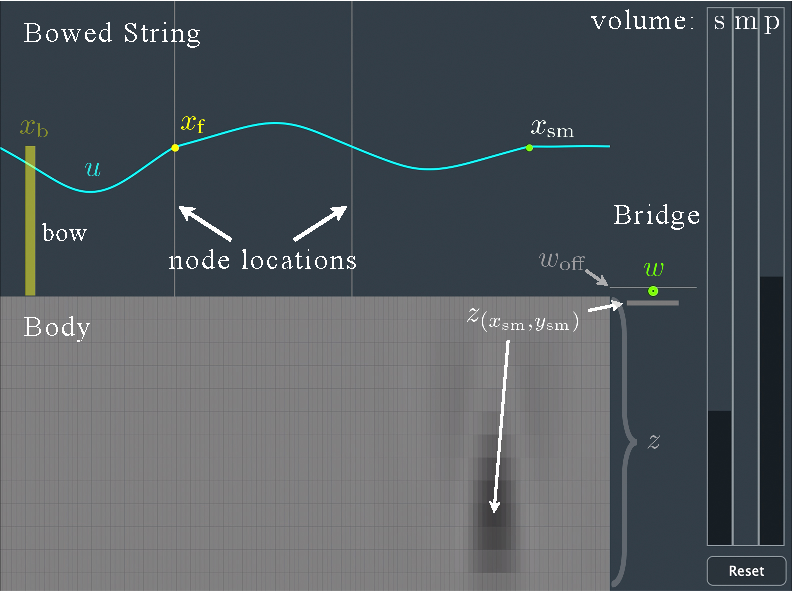
\includegraphics[width=1.0\columnwidth]{applicationDescription.pdf}
  \caption{The GUI showing the excited system with components highlighted. A more detailed description can be found in Section \ref{sec:GUI}. %\SWcomment[Same as in Figure 3, should I use $l_\text{f}, l_\text{sm}$, etc. instead of $x_\text{f}, x_\text{sm}$, etc.?]\SBcomment[I would just use the continuous variables for both figures...]
  }
  \label{fig:GUI}
\end{figure}
\subsection{Graphical User Interface}\label{sec:GUI}
A screenshot of the GUI is shown in Figure \ref{fig:GUI}. The GUI is divided in four sections, three showing the states of the string, bridge and body respectively and one control section. 

Firstly, the string section shows the state of the string $\us$ as a cyan-coloured path and the bow as a yellow rectangle with bow position $\stringx_\text{b}$ and its opacity depending on the bow force $F_\text{b}$. Furthermore, the bridge state $\um^n$ is shown as a green circle at location (of the bridge along the string) $\stringx_\text{sm}$. Finally, the position of the damping finger $\stringx_\text{f}$ is displayed as a yellow circle, the size of which depends on damping coefficient $\sigma_\text{f}$. The position of the finger triggers lines showing the locations of the closest nodes along the string according to the following equation
\begin{equation}\label{eq:node}
    \stringx_\text{node}^i = \frac{i\cdot \stringx_\text{sm}}{n}\quad \text{for} \quad i = [1,\hdots,n-1],
\end{equation}
where $n = \text{round} (\stringx_\text{sm}/\stringx_\text{f})$ is an integer closest to the ratio between the string length until the bridge location and the damping finger position. These lines are drawn to help the user place the damping finger at nodes along the string.

Secondly, the bridge section shows the displacement of the bridge $\um$ as a green circle, the state of the body at the collision location $\up_{(l_\text{sm},m_\text{sm})}$, both moving vertically according to their respective displacements and finally, a static grey horizontal line denoting the offset $\um_\text{off}$, i.e., the resting position of the bridge.

Thirdly, the body section shows the state of the body $\up$ as a grid of rectangles changing (grey-scale) colour according to their displacement.

Finally, the control section contains three sliders that control the volume-levels of the string (s), bridge (m) and body (p) respectively (for experimentation of volume ratios between the components) and a reset button to re-initialise the system. 

\subsection{Sensel Morph and Mapping}
The Sensel is an expressive touch controller using \texttildelow20,000 pressure-sensitive sensors laid out in an hexagonal grid \cite{sensel2020}. It retrieves x and y-positions and pressure at a rate of 150 Hz from which velocities and accelerations can be obtained.

The first finger registered by the Sensel is mapped to the bow: x-position is mapped to bow position $\stringx_\text{b}$, y-velocity to bow velocity $v_\text{b}$ (y-position is shown in the GUI but does not influence the model directly) and pressure to bow force $F_\text{b}$. The second finger is mapped to the damping finger: x-position is mapped to finger location $x_\text{f}$ and pressure to damping coefficient $\sigma_\text{f}$.

\section{Results and Discussion}\label{sec:resDisc}
%Figure \ref{fig:waveforms} shows the isolated outputs of the bridge and the body (at $(x_\text{mp},y_\text{mp})$) over time. %The string is bowed at $x_\text{b} = 0.3L$, with speed $v_\text{b} = 0.2$ and force $F_\text{b} = 0.1$ and damping finger position $x_\text{f} = 0.5x_\text{sm}$ and damping $\sigma_\text{f} = 0.1$ to induce the lowest harmonic. 
%Interestingly, compared with trombone measurements from \cite[Figure 6]{Boutin2015:SMC2020}, the bridge and the body exhibit similar patterns to the flow due to the lip motion through the bore and the pressure at the bore respectively. 
Informal listening by the authors has confirmed that the sound has brass-like qualities and comparison with the recreated tromba marina showed that the sound exhibited similar qualities. Naturally, formal listening tests need to be conducted to verify this.
% \begin{figure}[t]
%   \centering
%   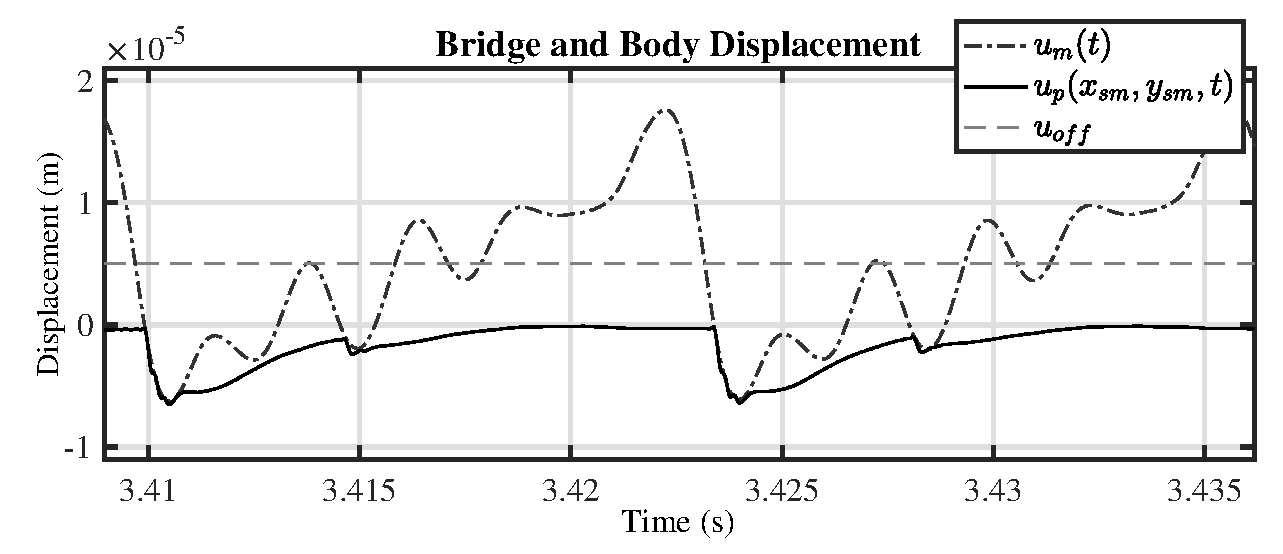
\includegraphics[width=\columnwidth]{trombaWaveforms2.eps}
%   \caption{The isolated outputs of the bridge and body (at collision location $(x_\text{mp},y_\text{mp})$) with bow parameters $\stringx_\text{b} = 0.3L$, $v_\text{b} = 0.2$, $F_\text{b} = 0.1$ and damping finger position $\stringx_\text{f} = 0.5\stringx_\text{sm}$ and damping $\sigma_\text{f} = 0.1$ to induce the lowest harmonic.}
%   \label{fig:waveforms}
% \end{figure}

Disabling the graphics of the application, its CPU usage is 68.9\% on a MacBook Pro with a 2.2 GHz Intel i7 processor, easily allowing it to work in real-time. As the heaviest part of the algorithm is the calculation of the body, the minimum grid spacing $h_{\text{p},\text{min}}$ could be set to a higher value to decrease the CPU usage. However, as mentioned, this will decrease the quality of the output sound.

Through using the application, the authors found some odd behaviour, where the bridge `gets stuck' behind the plate, i.e., values for $\psi_\text{mp}$ would be negative for a short period of time (one to several samples). The explicit technique used in this work allows for this to happen (and can be proven to still be stable in this case \cite{Ducceschi2019}), but it is `unphysical' to have a negative potential as this implies a `pulling' collision. As can be seen from Table \ref{tab:parameters}, the nonlinear collision coefficients $\alpha_\text{sm}$ and $\alpha_\text{mp}$ are set to $1$. When increasing these values, this behaviour would arise much more often, and even occur for a prolonged period of time (several seconds to indefinitely). This is also the reason why the reset button presented in Section \ref{sec:GUI} has been implemented%, to undo this negative potential
. As mentioned in \cite{Ducceschi2019}, oversampling increases the accuracy of the explicit collision method, and could be a solution to this issue. However, in order for the application to run in real time, this solution can not be afforded without decreasing the quality of the implementation, e.g. increasing $h_{\text{p},\text{min}}$. Further investigation will be necessary to solve this issue without oversampling.

Lastly, it has been found that when $|\up_{(l,m)}^n| \lessapprox 10^{-306}$ (but non-zero) for any coordinate $(l,m)$ (which happens when the body has not been collided with for a prolonged period of time), the CPU usage increases considerably. This could be explained by the fact that calculations with extremely small values are handled differently by the application.  %\SWcomment[Maybe we should ask Craig about this..] 
This is solved by implementing a limit to how small a value for $\up_{(l,m)}^n$ can be. If the value of $\up_{(l_\text{sm},m_\text{sm})}^n$ is lower than this limit, the total plate state is set to $0$. 

\section{Conclusion and Future Work}\label{sec:conclusion}
In this paper, a real-time implementation of a simulation of the tromba marina has been presented. The output sound has been found natural and brass-like by the authors and exhibited similar qualities when compared to a real (recreated) tromba marina.

Future work includes a comparison between the non-iterative methods used in this paper and iterative methods (such as and Newton-Raphson) both regarding algorithm speed and sound quality. 

Lastly, for a more physical implementation of the damping finger, it would be good to model it as another mass colliding with the string rather than directly imposing damping onto the string state.

\begin{acknowledgments}
The authors would like to thank Peter Williams for his valuable feedback on our application.

This work is supported by NordForsk's Nordic
University Hub Nordic Sound and Music Computing Network
NordicSMC, project number 86892. Ducceschi's work was supported by an Early Career Fellowship from the Leverhulme Trust.
\end{acknowledgments} 

%%%%%%%%%%%%%%%%%%%%%%%%%%%%%%%%%%%%%%%%%%%%%%%%%%%%%%%%%%%%%%%%%%%%%%%%%%%%%
%bibliography here
{%\small
\bibliography{smc2020bib}
}
\end{document}
